s
\section{Evaluation}
\label{sec:eval}

We evaluate the scalability of \ix and compare it to the Linux baseline
and to mTCP, the state-of-the-art user-space TCP alternative available
on the same hardware.  We first describe the experimental setup
(\S\ref{sec:eval:setup}).  We then characterize the performance using
a series of micro-benchmark: the popular NetPIPE ping-pong
test~\cite{snell1996netpipe} (\S\ref{sec:eval:netpipe}); the short
message transaction test previously used to evaluate
MegaPipe~\cite{han2012megapipe} and mTCP~\cite{jeong2014mtcp} in
\S\ref{sec:eval:short}; and the scalability of the system for large
persistent connections (\S\ref{sec:eval:scale}).  Finally, we
characterize the performance of the \ix system by running real-world
applications such as memcached and XXX using the
\texttt{libevent-}compatibility library(\S\ref{missing}).


\subsection{Experimental setup}
\label{sec:eval:setup}

\edb{Describes EPFL setup:}
Our experimental setup consists of a cluster of 19 clients and one
server connected by an HP 5820AF-24XG low-latency 10GbE switch.  The client
machines are a mix of dual Xenon E5-2637 running at 3.5 Ghz and single Xenon E5-2650 running at 2.6 Ghz with a single, Intel
82599EB 10GbE NIC connecting to the switch.  The server is a dual-Xeon E5-2665
running at 2.4 Ghz with 256 GB of DRAM with four Intel 2P X520 NICs.  Each
socket (client or server) has 8 cores and 16 hyperthreads.  When
reporting multi-core scalability, we report results with
hyperthreading enabled, and both hyperthreads of the cores are used.

For our experiments, the server is connected to
the switch via either a single 10GbE link or via a 4x10GbE bond configured as a L2+L3
hash via LACP~\cite{ieee802.3ad}. Jumbo
frames are never enabled.  Our baseline configuration in each machine
is the Ubuntu 12.04.4 LTS distribution running the 3.11.10 Linux kernel.  Although
the server has two sockets, our experiments pin IRQs\george{not really}, processes, and
the IX dataplane onto a single socket and use memory from that socket;
all NICs are attached to that socket via the PCIe root complex. 
\edb{CONTREVERSIAL: We chose to limit execution to a single NUMA node to simplify the
  analysis because of the asymmetrical nature of our hardware, to
  model the experimental setup after the one used in recent related
  work~\cite{jeong2014mtcp}, and also as we are practically never CPU-bound in our tests}

%\christos{We should organize the eval in the following way: first
%  micro-benchmarks that showcase each of the advantages (high packet
%  rate, low latency/jitter, high connection/churn). The title of the
%  subsection should indicate the aspect evaluated. Then there should
%  a subsection on full app eval (memcache hopefully).}

Whenever both practical and relevant, we compare the performance of an
\ix server with a baseline out-of-the-box Linux configuration
((\texttt{Linux-base}), an optimized configuration of Linux
(\texttt{Linux-opt}), and the performance of mTCP, a
recently-published user-level TCP stack specifically designed for
scalability~\cite{jeong2014mtcp}.  Unless specifically mentioned, all
clients run a baseline Linux configuration. 

The Linux server implementations use the
\texttt{libevent} framework running on XXX threads to serve the
clients. The mTCP server implementation use the native mTCP API
running on up to 8 cores (within each core, one hyperthread is
dedicated to processing the network stack).  We downloaded and installed mTCP \edb{vXXX} from the public-domain implementation~\cite{missing}, but re-wrote the benchmarks as they were not part of the distribution.
Finally, \ix server use
the native \ix API running on up to 8 cores (using symmetrically both
hyperthreads).  For all experiments, we use the same Linux client code, generally also written using \texttt{libevent}.


\subsection{High-bandwidth and low-latency}
\label{sec:eval:netpipe}

\begin{figure}
\begin{centering}
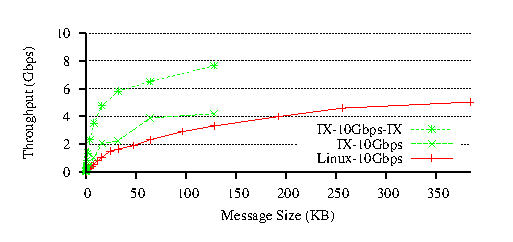
\includegraphics{figs/pingpong.eps}
\caption{NetPIPE performance for varying message sizes and system software configurations.}
\label{fig:pingpong}
\end{centering}
\end{figure}



%%%
%%%  use the ping-pong test to measure the half rountrip latency @ 64B
%%% 

\begin{table}[b]
\vspace{-1em}
\begin{center}
\begin{small}
\begin{tabular}{|l|c|c|}
\hline
Workload &  Avg lat. & 99\% lat. \\
\hline
Linux(base)-Linux(base)  & 60\microsecond & 0\microsecond\\
Linux(opt)-Linux(opt)    & 0\microsecond &  0\microsecond \\
mTCP-mTCP                & 0\microsecond &  0\microsecond \\
Linux(opt)-\ix           & 0\microsecond &  38\microsecond\\
\ix-\ix                  & 0\microsecond &  0\microsecond\\
\hline
\end{tabular}
\caption{Netpipe half-roundtrip latency (s=64B)}
\vspace*{-2em}
\label{tbl:pingpong}
\end{small}
\end{center}
\end{table}



We start the evaluation with the popular NetPIPE ping-pong
benchmark~\cite{snell1996netpipe} that exchanges a fixed-size message
between two servers.  The benchmark is used to calibrate the latency
and single-flow bandwidth of a communication link: with minimal
message size (64B), this benchmark determines the one-way latency for
short message communication.  With increasingly larger messages, it
determines how quickly this single ping-pong behavior can utilize 50\%
of the available bandwidth on the link.

Fig.~\ref{fig:pingpong} compares the performance of various
configurations for different message sizes and
Table~\ref{tbl:pingpong} additionally lists the average and 99\%
latencies for 64B messages, as well as the minimal message size
required to exceed 5Gbps of bandwidth.  Going from Linux to \ix saves
\twiddle 15\microsecond on each end.  When both ends are running \ix,
the end-to-end latency is reduced by two-thirds to 17\microsecond.
Similarily, the bandwidth increases much faster with \ix. \edb{TODO - Based on data}

\edb{THE LATENCY OF 17\microsecond IS UNDERWHELMING -- FAST PATHING IT SHOULD HELP}

\subsection{Handling high TCP connection churn}
\label{sec:eval:short}


%% put the key last to have correct numbering

\begin{figure*}[t]

\centering
  \vspace*{0.3in}
 \subfloat[Multi-core scalability (n=1;s=64B)]{
  \label{fig:short:mcore}
   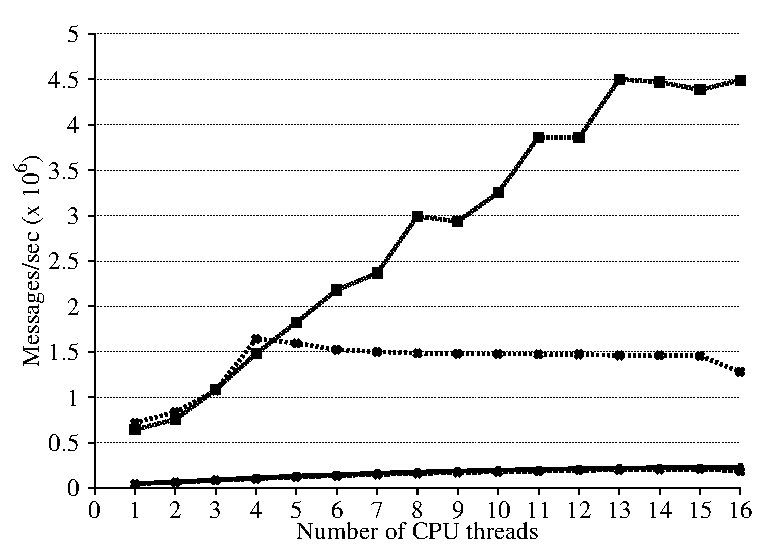
\includegraphics{figs/short-mcore.eps}}
 \hspace{.01in}
 \subfloat[$n$ roundtrips per conn. (core=8,s=64B)]{
  \label{fig:short:roundtrips}
  
\includegraphics{figs/short-roundtrips.eps}}
  \hspace{.01in}
 \subfloat[Different message sizes $s$ (core=8,n=1)]{
  \label{fig:short:size}
  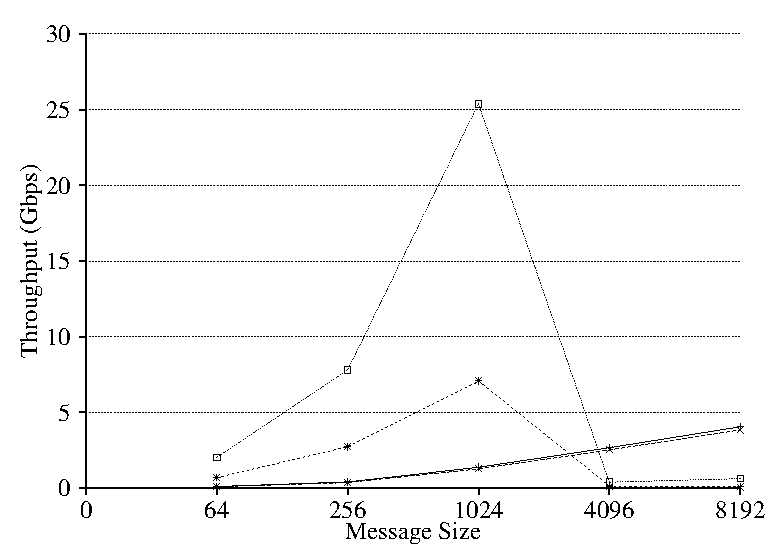
\includegraphics{figs/short-size.eps}}
 \centering
  \vspace{-1.9in}
  \subfloat{
\includegraphics{figs/short-key.eps}}
 \vspace{1.5in}
 \
\caption{Short message performance.}
 \label{fig:short}

\end{figure*}


We then evaluate \ix's multi-core scalability in handling workloads
with extreme connection churn by using the same benchmark used to evaluate
Megapipe~\cite{han2012megapipe} and mTCP~\cite{jeong2014mtcp}:
multiple clients connect to a single server listening on a single
port, send a request of size $s$ and wait for an echo of a message of
the same size.  As with NetPIPE, while accepting the message, the server holds off its
echo response until the message has been entirely received.
Each client performs this synchronous remote procedure
call $n$ times, and then close the connection using a reset
(\texttt{TCP RST}).


\edb{PLACEHOLDER:} Fig.~\ref{fig:short} shows the results for both
10GbE and 4x10GbE hardware configurations.  We first
are able to confirm and reproduce the mTCP performance published in
~\cite{jeong2014mtcp}.  On this benchmark, \ix generally scales XXx
better than mTCP on a per core basis and XXx better than Linux.  In
Fig.~\ref{fig:short:mcore}, we see that \ix can saturate the single
10Gbpe wire using only 3 cores; in contrast mTCP requires all 8
cores. \ix can further scale to nearly XX\% of the wire limit on a
4x10GbE configuration, and using a single socket.
Fig.~\ref{fig:short:roundtrips}, which uses 8 cores, similarly shows
that \ix can nearly saturate the wire on the single-link
configuration, but remains CPU-bound on the 4x10 configuration.
Finally, Fig.~\ref{fig:short:size} shows that only \ix can saturate
4x10Gbps with 4KB messages, and only \ix and mTCP can saturate the
single-link configuration.


\subsection{Connection Scalability}



%FIXME if different keys


\begin{figure*}[t]

\centering
  \vspace*{0.3in}
 \subfloat[Throughput for varying established connections]{
  \label{fig:connscaling:throughput}
   
\includegraphics[width=.49\textwidth,clip]{figs/blank.eps}}
 \hspace{.02in}
 \subfloat[Avg. and 99\% latency for varying established connections]{
  \label{fig:connscaling:lat}
  
\includegraphics[width=.49\textwidth,clip]{figs/blank.eps}}
\centering
  \vspace{-2.8in}
  \subfloat{
\includegraphics[width=1\textwidth,clip]{figs/short-key.eps}}
 \vspace{2.3in}
 \
\caption{Connection scaling}
 \label{fig:connscaling}

\end{figure*}

\label{sec:eval:scale}

We now evaluate \ix's scalability when handling a large number of
concurrent connections. In this benchmark, each client machine runs
$n$ threads, with each thread independently performing a 64B remote
procedure call to the server.  Each RPC randomly chooses among $m$
open sockets to perform the RPC.  In our setup with 18 clients, the
server must multiplex among $18 \times n \times m$ open connections.
We experimentally set $n \leq 24$ to maximize throughput.  The 19th
client performs RPC at a low rate on a single connection to measure
latency.  We report the throughput in message per second and the
round-trip latency for varying number of total established connections.

Fig.~\ref{fig:connscaling} shows the results.  As expected, throughput
increases with the degree of concurrency, but then decreases with
increasing number of connections due to the increasingly high cost of
multiplexing among open connections.  At the peak, \ix performs XXx
better than Linux, consistent with the results from
Fig.~\ref{fig:short:roundtrips}.  With 100,000 connections, \ix is
able to deliver XX\% of its peak throughput, whereas Linux only
delivers XXX\% of its own peak throughput\footnote{Unexplained
  performance issues with our client configuration setup limit our
  experiments to 100,000 connections at the time of submission. \ix is
  designed to scale to millions of concurrent connections.}


\subsection{Application performance -- memcache}
\label{sec:eval:memcache}

\todo Compare apples-to-apples with Megapipe, and mTCP in terms of microbenchmarks.

\todo Baseline comparison of state-of-the art systems include:  Linux (some recent version, with SO\_REUSEPORT); Megapipe (if possible), mTCP (if possible). 

\todo Microbenchmark: short TCP transactions (echo server, as defined in megapipe).   Goal is to beat mTCP (and therefore all others) hands down.

\todo Benchmark: memcached - compare with FB results (?)

\todo Benchmark: lightttpd -- used by Affinity-Accept and mTCP.  

\todo ngnx: an actually used webserver.


%%%%%
%%%%% very optimistic
%%%%%


\subsection{Multi-tier Performance}

\edb{THIS IS A STRECH STRETCH GOAL} 

Evaluating the performance of a highly-scalable, multi-tier
environment in a lab environment is challenging on multiple fronts:
first, there are ---to the best of our knowledge--- no universally
accepted multi-tier benchmarks that involve key-value stores and in
general that are representative of web-scale applications.  Second,
most lab enviornments are orders of magnitude smaller than a
datacenter.

Therefore, we construct a simple, synthetic multi-tier benchmark that
mimics the behavior of a social application stored in an in-memory
key-value store.  The application is a simple \texttt{http} server
that returns the top-most recent update among a users list of friends.
The application server parses the http request to
get the userid, uses the user id to return a friends-list from a
key-value store, and then queries the key-value store individually for
each friend for the most recent value.  It then processes replies and
return the top-most entries.  In our experiments, we model a database
with $10^7$ million users, each with 100 friends. 

We scale the benchmark to model a cluster deployment with $\alpha$
client connections per application server, $\beta$ httpd and $\gamma$
memcached servers.  Keys are distributed uniformly between the
$\gamma$ servers.  We model a large-scale deployment with
$\alpha=10^5$, $\beta=10^4$ and $\gamma=10^4$ on a deployment that consists of 4
actual application servers and 1 memcached server (running on our
server hardware with 4x10GbE connectivity).  Each application server
runs \texttt{lighthttpd} with the application logic written directly
within the server, and maintains a distinct connection for each of the
$\alpha$ virtual clients and $\gamma$ virtual nodes.  The key-value store is
running \texttt{memcache} as described in \S\ref{sec:eval:memcache}.
We use the remaining 14 client machines to simulate $4 \times \alpha$
clients and the 19th client to measure the latency of the application.

Fig.~\ref{missing} reports the latency as a function of the
throughput, as determined by varying the client load.  We compare a
Linux baseline with one in which \ix is used to run both the
application server and the memcached server.  We note that the choice
of operating system on the application server determines the number of
concurrent connections. Indeed, because of the coherence-free
execution model, each application server needs to open a distinct TCP
flow to the same virtual node for each of its hardware threads.

\edb{OPTIMISTIC: } Fig.~\ref{missing} shows that \ix can saturate the
hardware connectivity.  Indeed, the bottlneck consits of the
communication 





